%!TEX root = main.tex
\section{Vague Intelligent Search\label{sec:vague}}
Accounting for user interaction, mental models. More global objective taking into account user with the goal of dataset understanding rather than task completion.
\subsection{Challenges}
\begin{itemize}
\item Inferring user intent in querying and context is important (both in terms of user input and what is recommended)
\item tools can not assume user has querying intention. exploration without intention, user don’t know what they are searching for --> Recommendation.
\item The important thing here is identifying what should be done by the system v.s. requested from user. Inappropriate choice of these will result in lack of expressibility and user feeling lack of control of analysis, limiting exploration.
\item Need for a unified framework of inference to take all of these into account (e.g. natural language, etc)
\end{itemize}
\subsection{\sbd: Navigating Through Data Slices with Hierarchical Summary of Visualizations}

\begin{figure}[h!]
\label{fig:modalities}
\centering
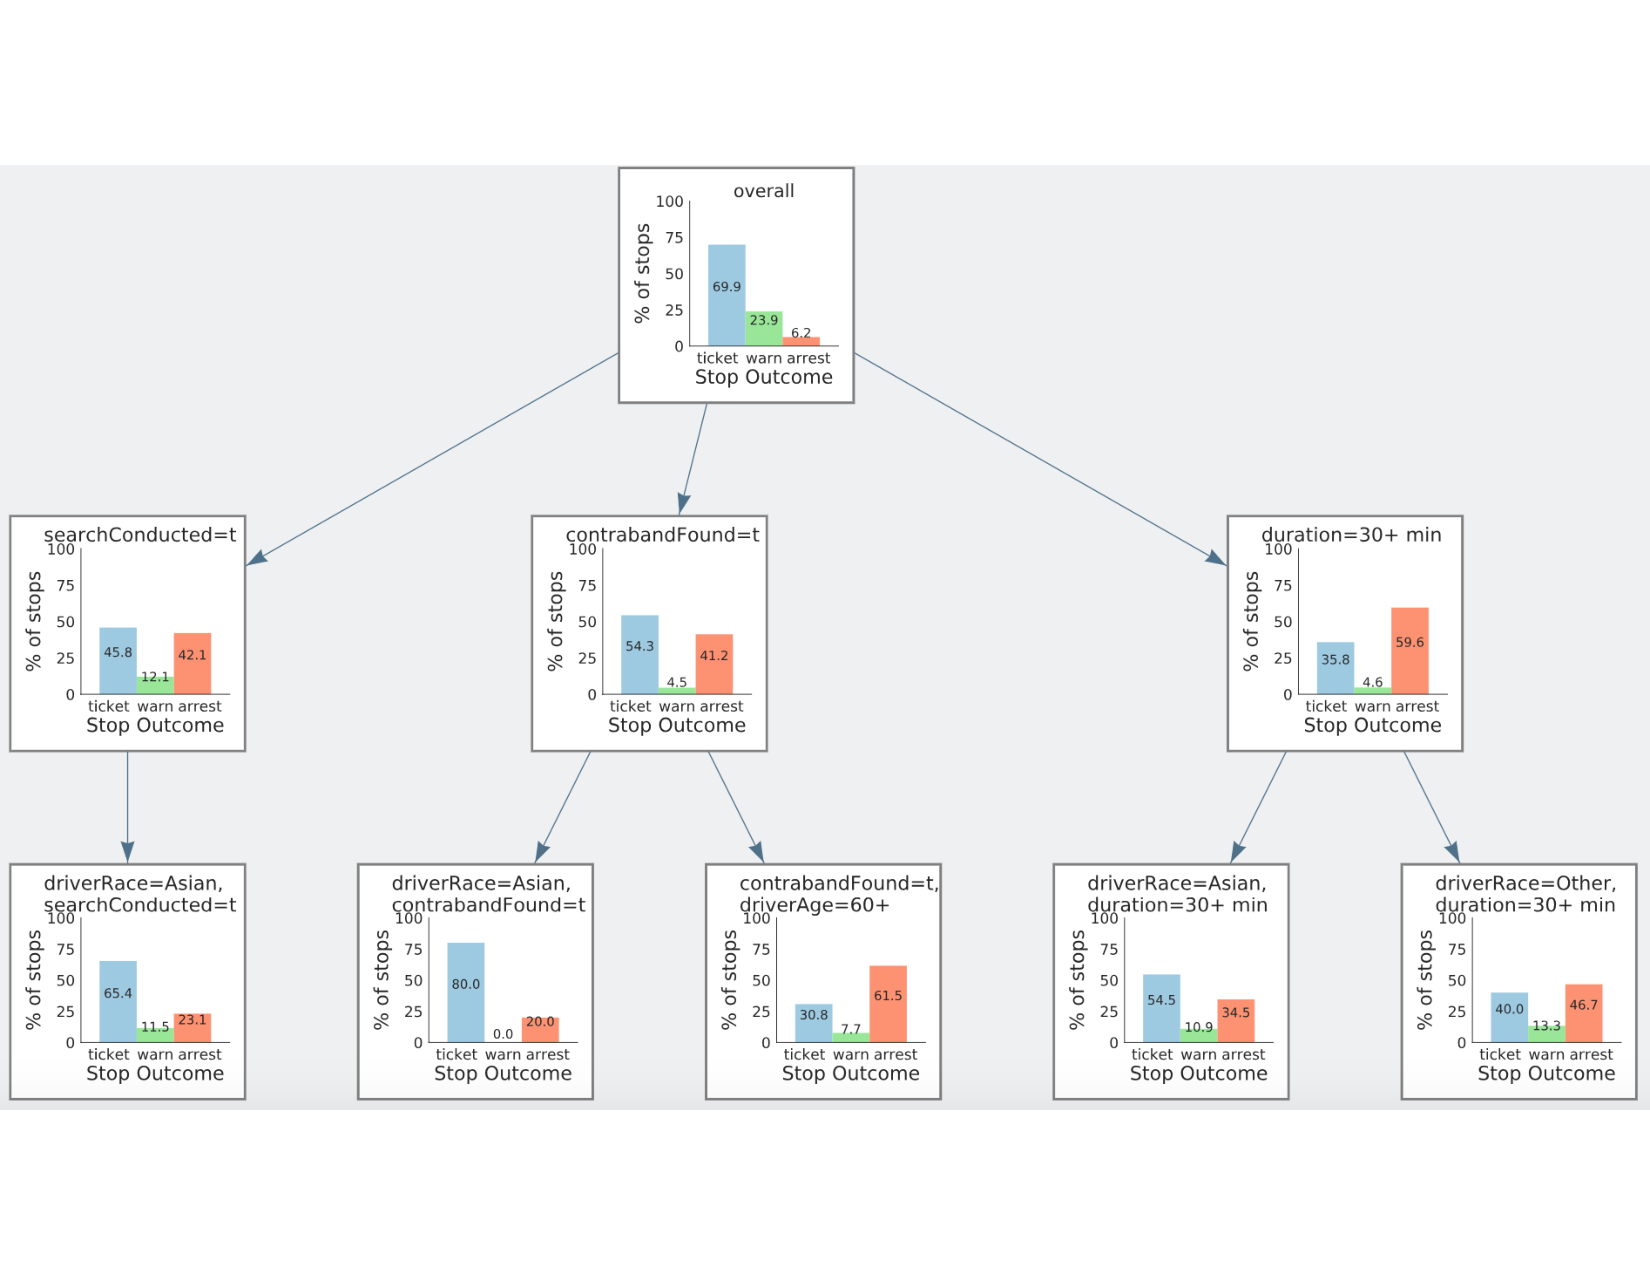
\includegraphics[width=0.7\linewidth]{figures/storyboard.pdf}
\caption{Example dashboard with generated from the Police Stop Dataset \cite{police}, which contains records of police stops that resulted in a warning, ticket, or an arrest.The attributes in the dataset include driver gender, age, race, and the stop time of day, whether a search was conducted, and whether contraband was found. We generate a dashboard of visualizations with bar charts with x-axis as the stop outcome (whether the police stop resulted in a ticket, warning, or arrest/summons) and y-axis as the percentage of police stops that led to this outcome.}
\end{figure}

Data is agnostic to the user, intention ---, by building tools---, Section \ref{sec:precise} to \ref{sec:vague} have focussed on extracting what user want from data. bridging together what user want from data, what data has to offer, supporting interactive discourse between the two. 
 Either using one-size-fits-all statistics, templates, heuristics as a solution or problem only applicable to a subset of analytic tasks\cite{Vartak2015,Vartak2017}. 